\chapter{Cost-benefit considerations in the growth of networks}
\label{chap:cost-benefit}

\section{A cost-benefit model for the growth of spatial networks}
\label{sec:a_cost_benefit_model_for_the_growth_of_spatial_networks}

\section{Scaling in transportation networks}
\label{sec:scaling_in_transportation_networks}


Almost $200$ subway systems run through the largest agglomerations in the world
and offer an efficient alternative to congested road networks in urban areas.
Previous studies have explored the topological and geometrical static properties
of these transit systems~\cite{Derrible:2009,Levinson:2012}, as well as their
evolution in time~\cite{Roth:2012}. However, subways are not mere geometrical
structures growing in empty space: they are usually embedded in large, highly
congested urban areas and it seems plausible that some properties of these
systems find their origin in the interaction with the city they are in. Previous
studies~\cite{Levinson:2008,Xie:2009} have shown that the growth and properties
of transportation networks are tightly linked to the characteristics of urban
environment. Levinson \cite{Levinson:2008} for instance, showed that rail
development in London followed a logic of both `induced supply' and `induced
demand'. In other words, while the development of rail systems within cities
answers a need for transportation between different areas, this development also
has an impact on the organisation of the city. Therefore, while the growth of
transportation cannot be understood without considering the underlying city, the
development of the city cannot be understood without considering the
transportation networks that run through it. As a result, the subway system and
the city can be thought as two systems exhibiting a symbiotic behaviour.
Understanding this behaviour is crucial if we want to get a deeper understanding
of how the city grows and how the mobility patterns organise themselves in urban
environments.

At a different scale, railway networks answer a need for fast transportation
between different urban centers. We therefore expect their properties to be
linked to the characteristics of the underlying country. A model of growth as
been recently proposed~\cite{Louf:2013}, and relates the existence of a given
line to the economical and geographical features of the environment. An
interesting question is thus to know whether subways and railway networks behave
in the same way, but at different scales. In other words, we are interested to
know whether subways are merely scaled down railway networks, or whether they
are fundamentally different objects, following different growth mechanisms. 

In the spirit of the model proposed in~\cite{Louf:2013}, we propose here a
large-scale framework which relates structural and economical properties of
subway and railway networks. Although many
studies~\cite{Kansky:1963,Derrible:2009,Levinson:2012} explore the interplay
between regional characteristics and the structure of transportation networks, a
simple picture relating the network's most basic quantities and the region's
properties is still lacking. It has been found that several biological and
man-made systems exhibit allometric scaling relationships between the output of
processes and size. These relationships are hints that very general processes
are at stake in the growth of these systems, and a first step towards their
understanding is to uncover these processes~\cite{Banavar:1999,Louf:2014}. In
the spirit of what has recently been done for cities~\cite{Louf:2014}, we try in
the following to understand the way subways and railway networks scale with some
of the substrates' most basic attributes: population, surface area and wealth. 

We believe this should lay the foundations for more specific and involved discussions.

As a result, we are able to relate the total ridership, the number of stations,
the length of the network to socio-economical features of the environment. We
find that these relations are in good agreement with the data gathered for $138$
subway systems and $58$ railway networks accross the world. In particular, we
show that even if the main mechanisms are the same, the difference of scale at
which both systems operate is responsible for their different behavior. 


% Results and Discussion can be combined.
\section*{Results}

\subsection*{Framework}

A transportation network is at least characterized by its total number of nodes
(which are here train or subway stations), its total length, and the total
(yearly) ridership. On the other hand, a city (or a country in the railway case)
is characterized by its area, its population and its GDP. Because transportation
systems do not grow in empty space, but result from multiple interactions with
the substrate, an important question is how network characteristics and
socio-economical indicators relate to each other. Naturally, cost-benefit
analysis seems to be the appropriate theoretical framework. While this approach
has already been developed in the context of the growth of railway
networks~\cite{Black:1971,Louf:2013}, these studies considered an iterative
growth: at each step an edge $e$ is built such that the cost function

\begin{equation} Z_e = B_e - C_e \end{equation}

is maximum. The quantity $B_e$ is the expected benefit and $C_e$ the expected
cost of $e$. In the following, we consider networks after they have been built,
and we assume that they are in a `steady-state' for which we can write a cost
function of the form

\begin{equation} Z =\sum_eZ_e= B - C \end{equation}

where $B$ is the total expected benefits and $C$ the total expected costs, now
operating costs (mainly maintenance costs). We further assume that, during this
steady-state, operating costs are balanced by benefits. In other words


\begin{equation} 
    Z \approx 0 
\end{equation} 

Indeed, because lines and stations cost money to be maintained, we expect the
network to adapt to the way it is being used. Therefore we can reasonably expect
that at first order the cost of operating the system is compensated by the
benefits gained from its use.  In the following we will apply this general
framework to subway and railway networks in order to determine the behavior of
various quantities with respect to population and GDP.

\subsection*{Subways}

In the case of subways, the total benefits in the steady-state are simply connected to the total ridership $R$ and the ticket price $f$ over a given period of time. The costs, on the other hand, are due to the maintenance costs of the lines and stations, so that we can write (for a given period of time)

\begin{equation}
    Z_{sub} = R\,f - \epsilon_L L - \epsilon_S N_s
    \label{eq:cost-benefit}
\end{equation}

where $L$ is the total length of the network, $\epsilon_L$ the maintenance cost of a line per unit of length, $N_S$ the total number of stations and $\epsilon_S$ the maintenance cost of a station (for a given period time).

It is usually difficult to estimate the ridership of a system given its characteristics and those of the underlying city. Due to the importance of such estimates for planning purposes, the problem of estimating the number of boardings per station given the properties of the area surrounding the stations has been the subject of numerous studies~\cite{Matsunaka:2013,Kuby:2004}. Here we are interested in the dependence of global, average behaviours of the ridership on the network and the underlying city. Very generally, we write that the number $R_i$ of people using the station $i$ will be a function of the area $C_i$ serviced by this station --- the `coverage'~\cite{Derrible:2009} --- and of the population density $\rho = \frac{P}{A}$ in the city

\begin{equation}
    R_i = \xi_i\, C_i\, \rho
\end{equation}

where $\xi_i$ is a random number of order one representing the ratio of people covered who use the subway. The main difficulty is in finding the expression of the coverage. It depends, a priori, on local particularities such as the accessibility of the station, and should thus vary from one station to another. We take here a simple approach and assume that on average

\begin{equation}
    C_i \sim \pi\, d_0^{\,2}
\end{equation}

where  $d_0$ is the typical size of the attraction basin of a given station. If we assume that it is constant, the total ridership can be written as

\begin{equation}
    R = \sum_i R_i \sim \overline{\xi} \pi d_0^2 \rho \: N_s
    \label{eq:ridership}
\end{equation}

where $\overline{\xi} = \frac{1}{N_s}\,\sum_i \xi_i$ is of the order of 1.\\

We gathered the relevant data for $138$ metro systems across the world (see
Materials and Methods), which we cross-verified when possible with the data
given by network operators. We plot the ridership $R$ as function of $N_s\,\rho$
on Fig.~\ref{fig:metro_ridership} and observe that the data is consistent with a
linear behavior. We measure a slope of $800\, \text{km}^2/\text{year}$ which
gives an estimate for $d_0$

\begin{figure}
\centering
    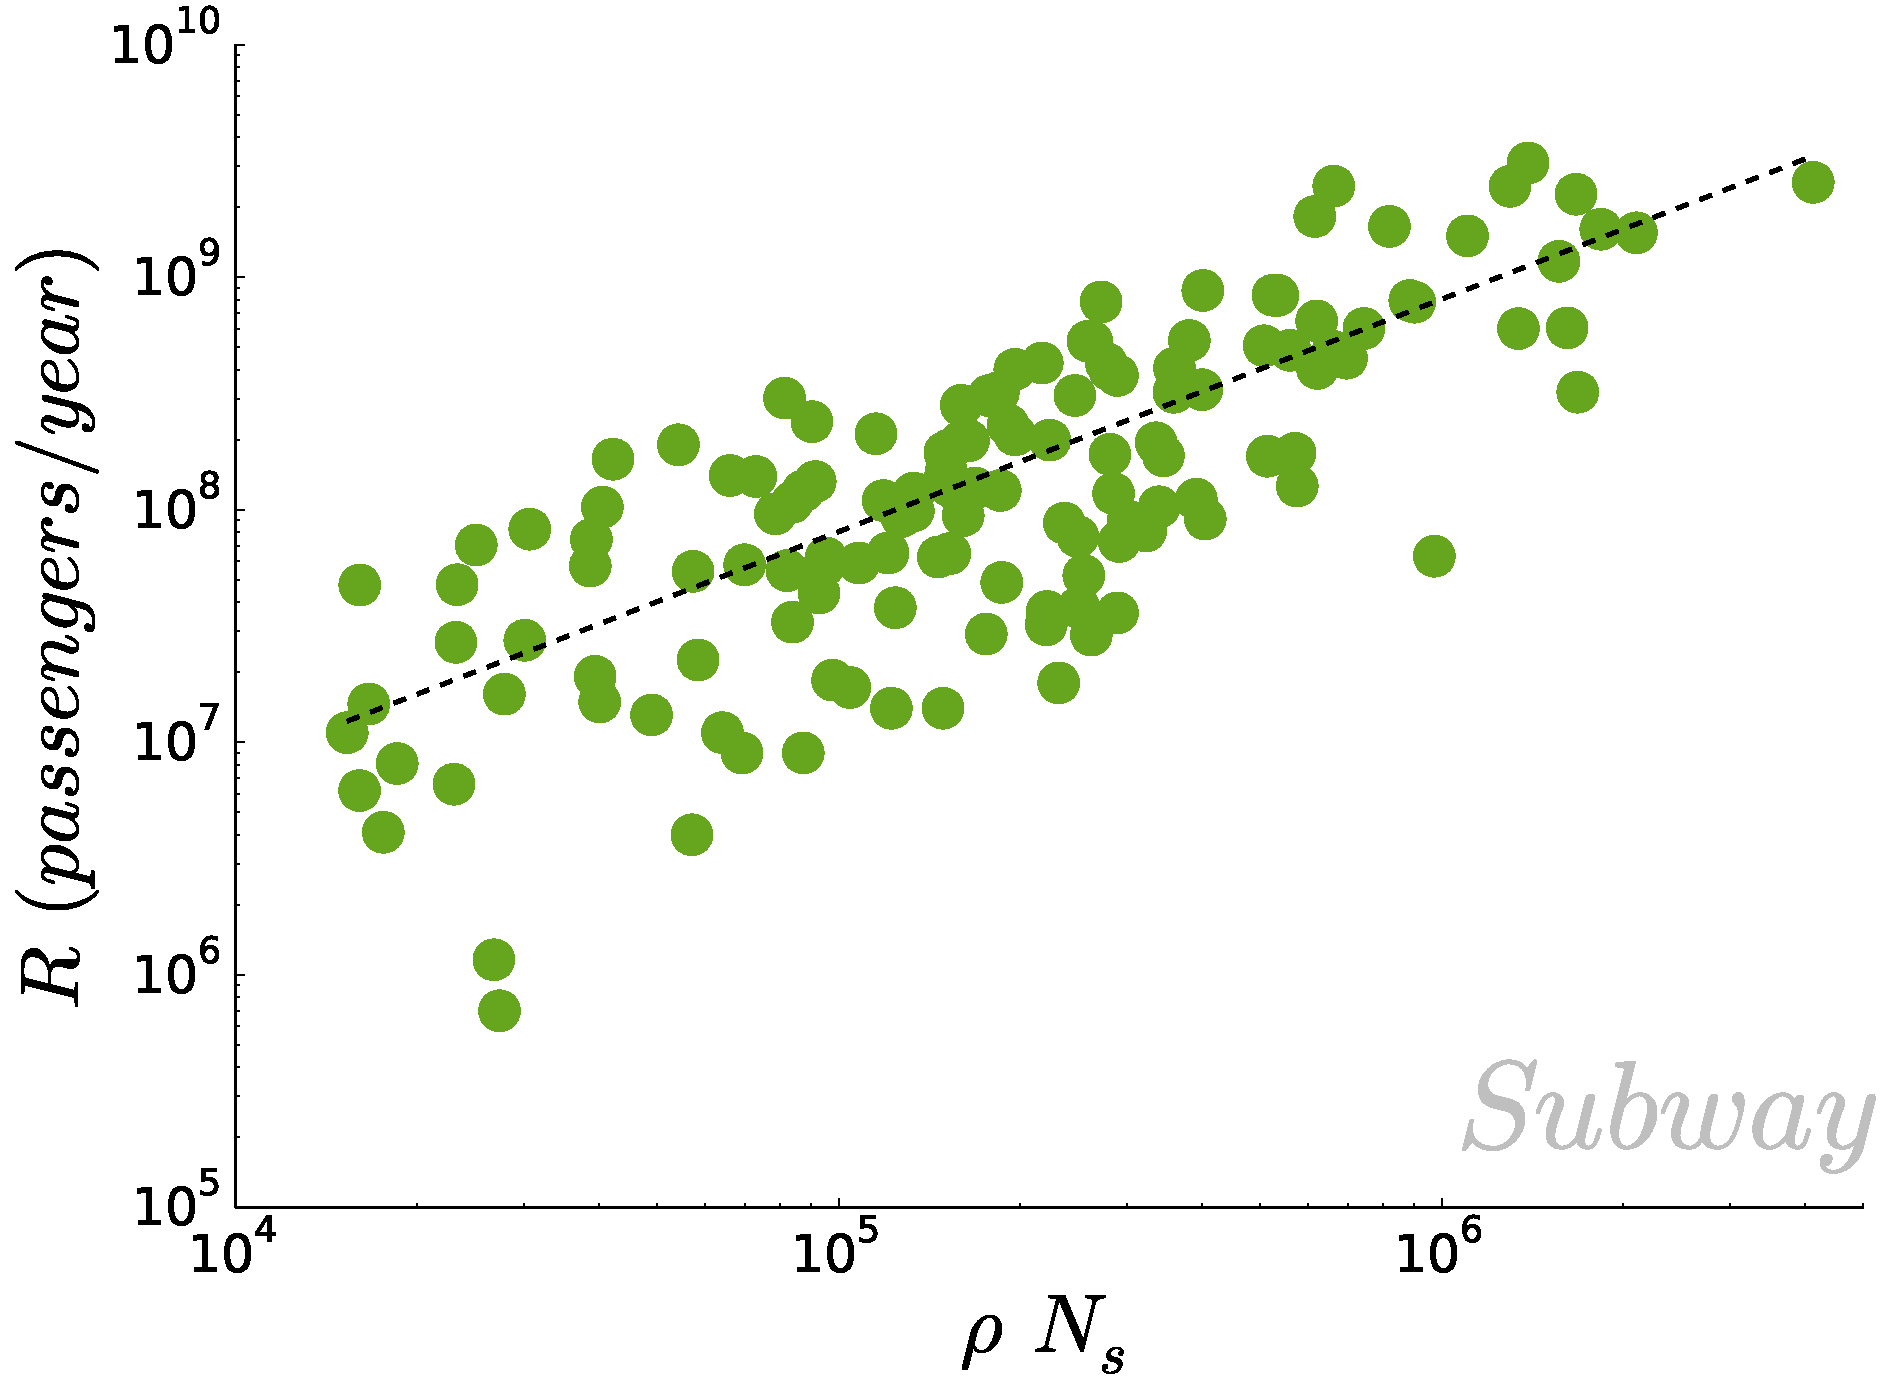
\includegraphics[width=.49\textwidth]{gfx/chapter-networks/metro_ridership_coverage.pdf}
    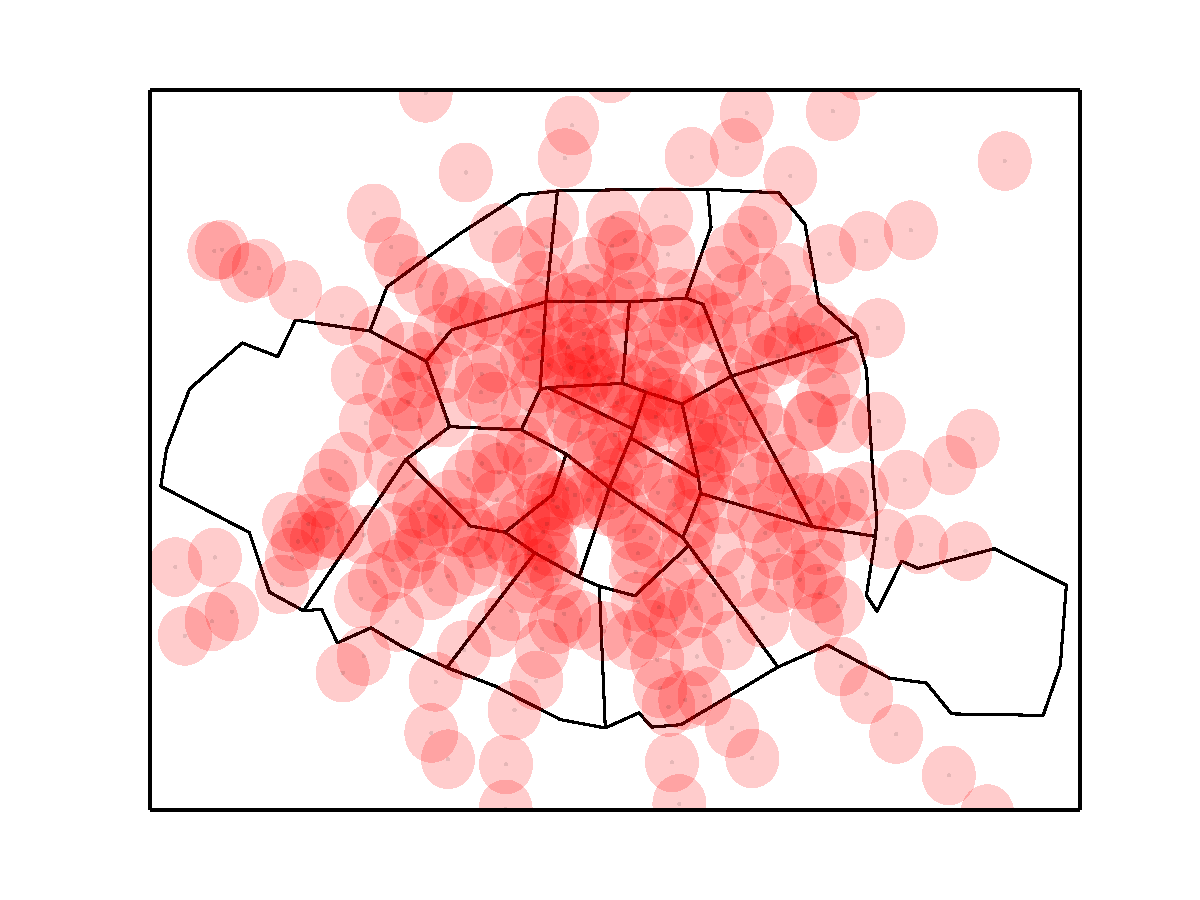
\includegraphics[width=.49\textwidth]{gfx/chapter-networks/paris_coverage.pdf}
    \caption{{\bf (Subway) The relationship between ridership and coverage} (Left)
    We plot the total yearly ridership $R$ as a function of $\rho\,N_s$. A linear
    fit on the $138$ data points gives $R \approx 800\:\rho N_s$ ($R^2=0.76$) which
    leads to a typical effective length of attraction $d_0 \approx 500\,\text{m}$
    per station. (Right) Map of Paris (France) with each subway station represented
    by a red circle of radius $500\,\text{m}$.\label{fig:metro_ridership}}
\end{figure}

\begin{equation}
    d_0 \approx 500\,\text{m}
\end{equation}

We illustrate this result on Fig.~\ref{fig:metro_ridership} by representing the
subway stations of Paris each with a circle of radius $500\,\text{m}$. 

So far, the distance $d_0$ appears here an intrinsic feature of user's
behaviors: it is the maximal distance that an individual would walk to go to a
subway station.

The average interstation distance $\ell_1$ is another distance characteristic of
the subway system. Rigorously, this distance depends on the average degree $<k>$
of the network so that $\ell_1 = \frac{2\,L}{N_s <k>}$. It has however been
found that for the $13$ largest subway systems in the world, $<k> \in
\left[2.1,2.4\right]$, so that we can reasonably take $<k> / 2 \approx 1$ and
thus

\begin{equation} \ell_1 \simeq \frac{L}{N_s} \end{equation}

The interstation distance depends in general on many technological and
economical parameters, but we expect that for a properly designed system it will
match human constraints. Indeed, if $d_0\ll\ell_1$, the network is not dense
enough and in the opposite case $d_0\gg\ell_1$, the system is not economically
interesting. We can thus reasonably expect that the interstation distance
fluctuates slightly around an average value given by twice the typical station
attraction distance $d_0$

\begin{equation} d_0 = \frac{\ell_1}{2} = \frac{L}{2\,N_s} \end{equation}

It follows from this assumption that the interstation distance is constant and
independent from  the population size. We plot on
Fig.~\ref{fig:metro_length_stations} the total length of subway networks as a
function of the number of stations. The data agrees well with a linear fit $L
\sim 1.13\,N_S\,(r^2=0.93)$. We also plot on
Fig.~\ref{fig:metro_length_stations} the histogram of the inter-station length,
showing that the interstation distance is indeed narrowly distributed around an
average value $\overline{\ell_1} \approx 1.2\,\text{km}$ with a variance $\sigma
\approx 400\,\text{m}$, consistently with the value found above for $d_0\approx
500\,\text{m}$. The outliers are San Francisco, whose subway system is more of a
suburban rail service and Dalian, a very large city whose metro system is very
young and still under development.

\begin{figure}
    \centering
    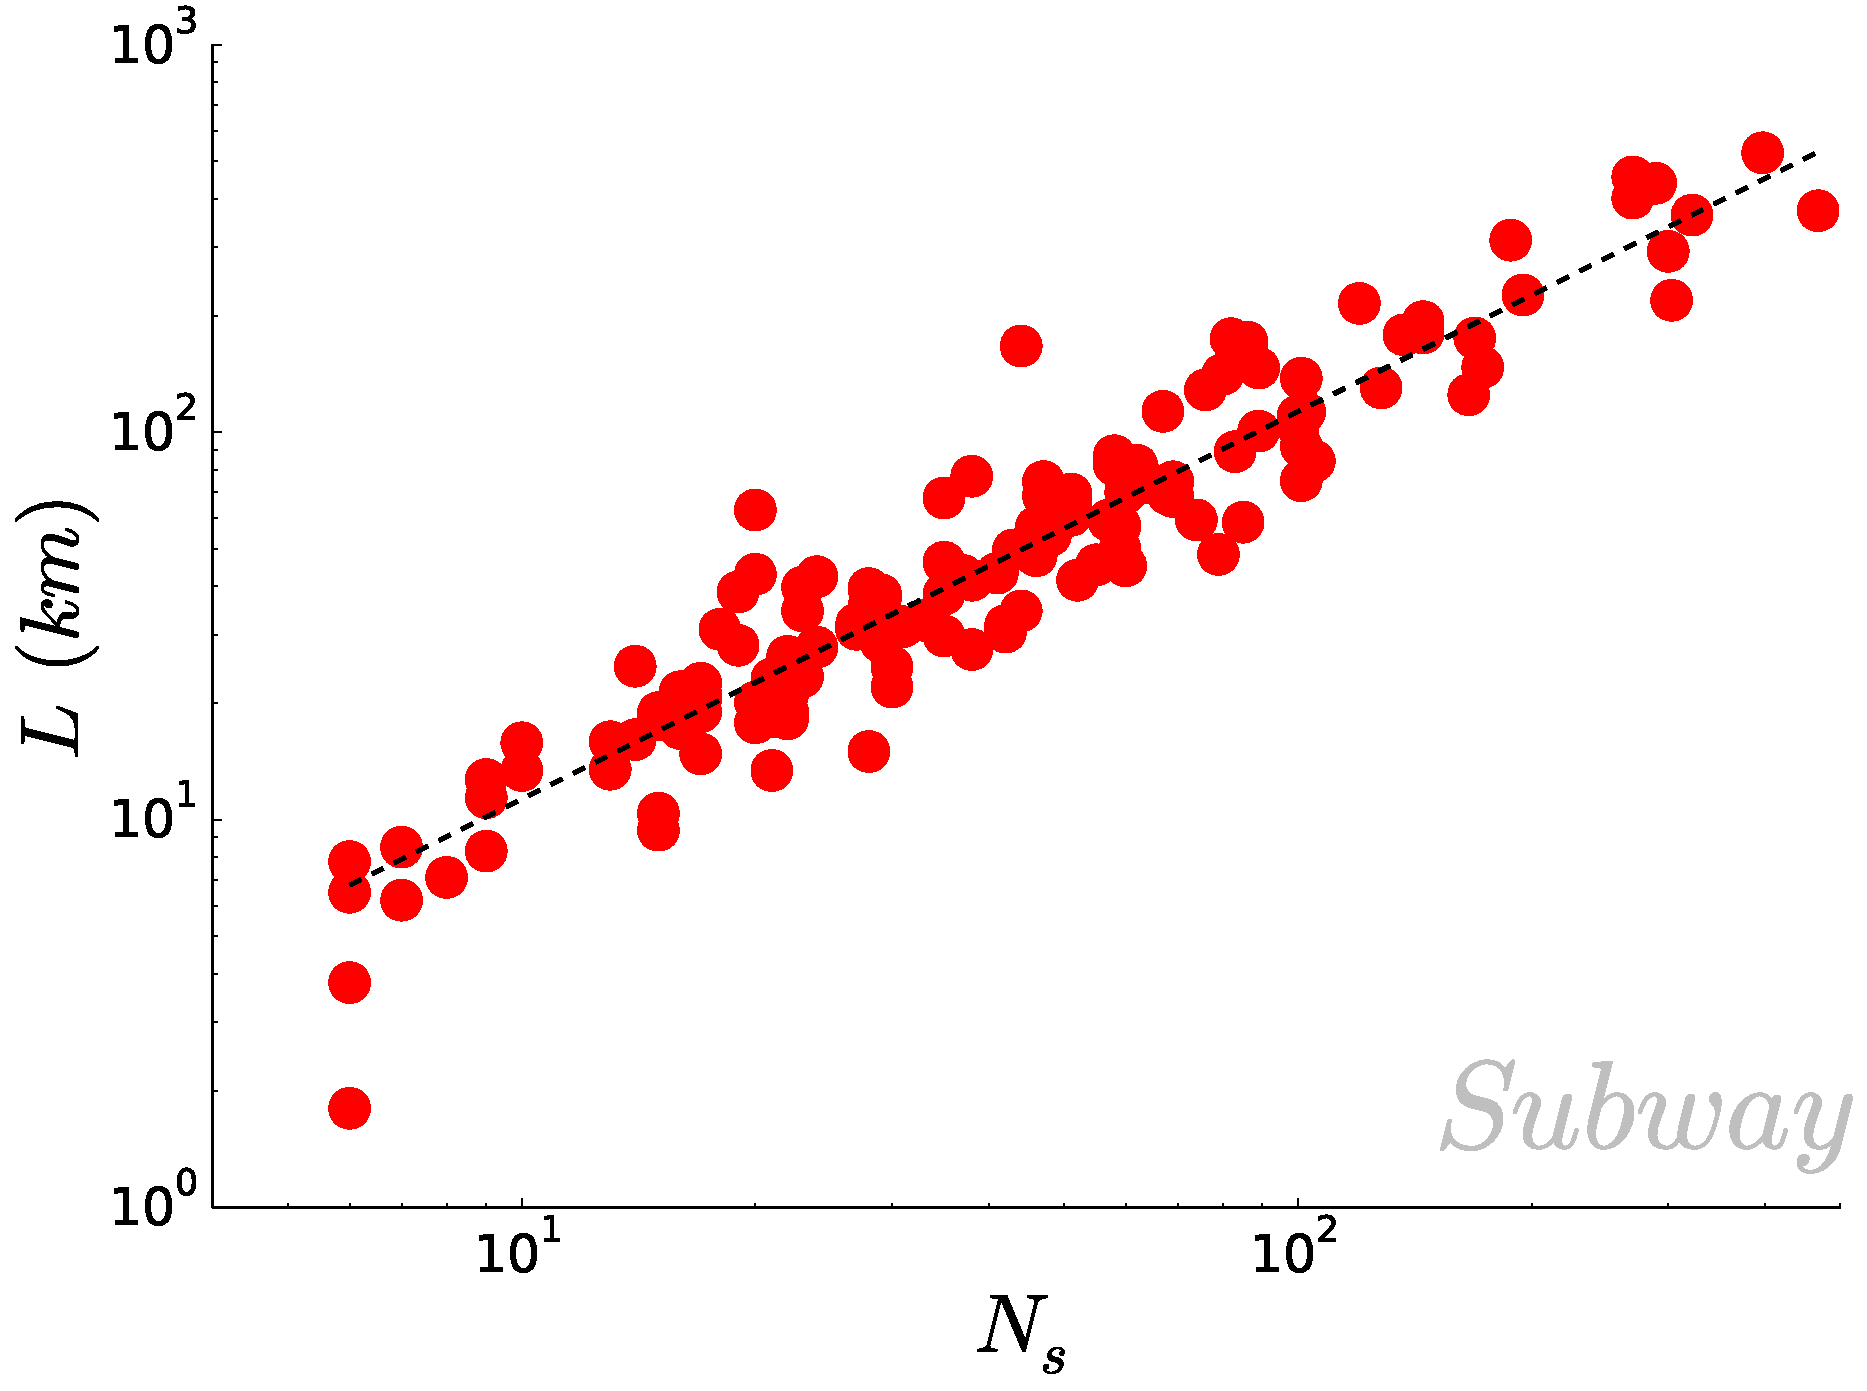
\includegraphics[width=0.49\textwidth]{gfx/chapter-networks/metro_length_stations.pdf}
    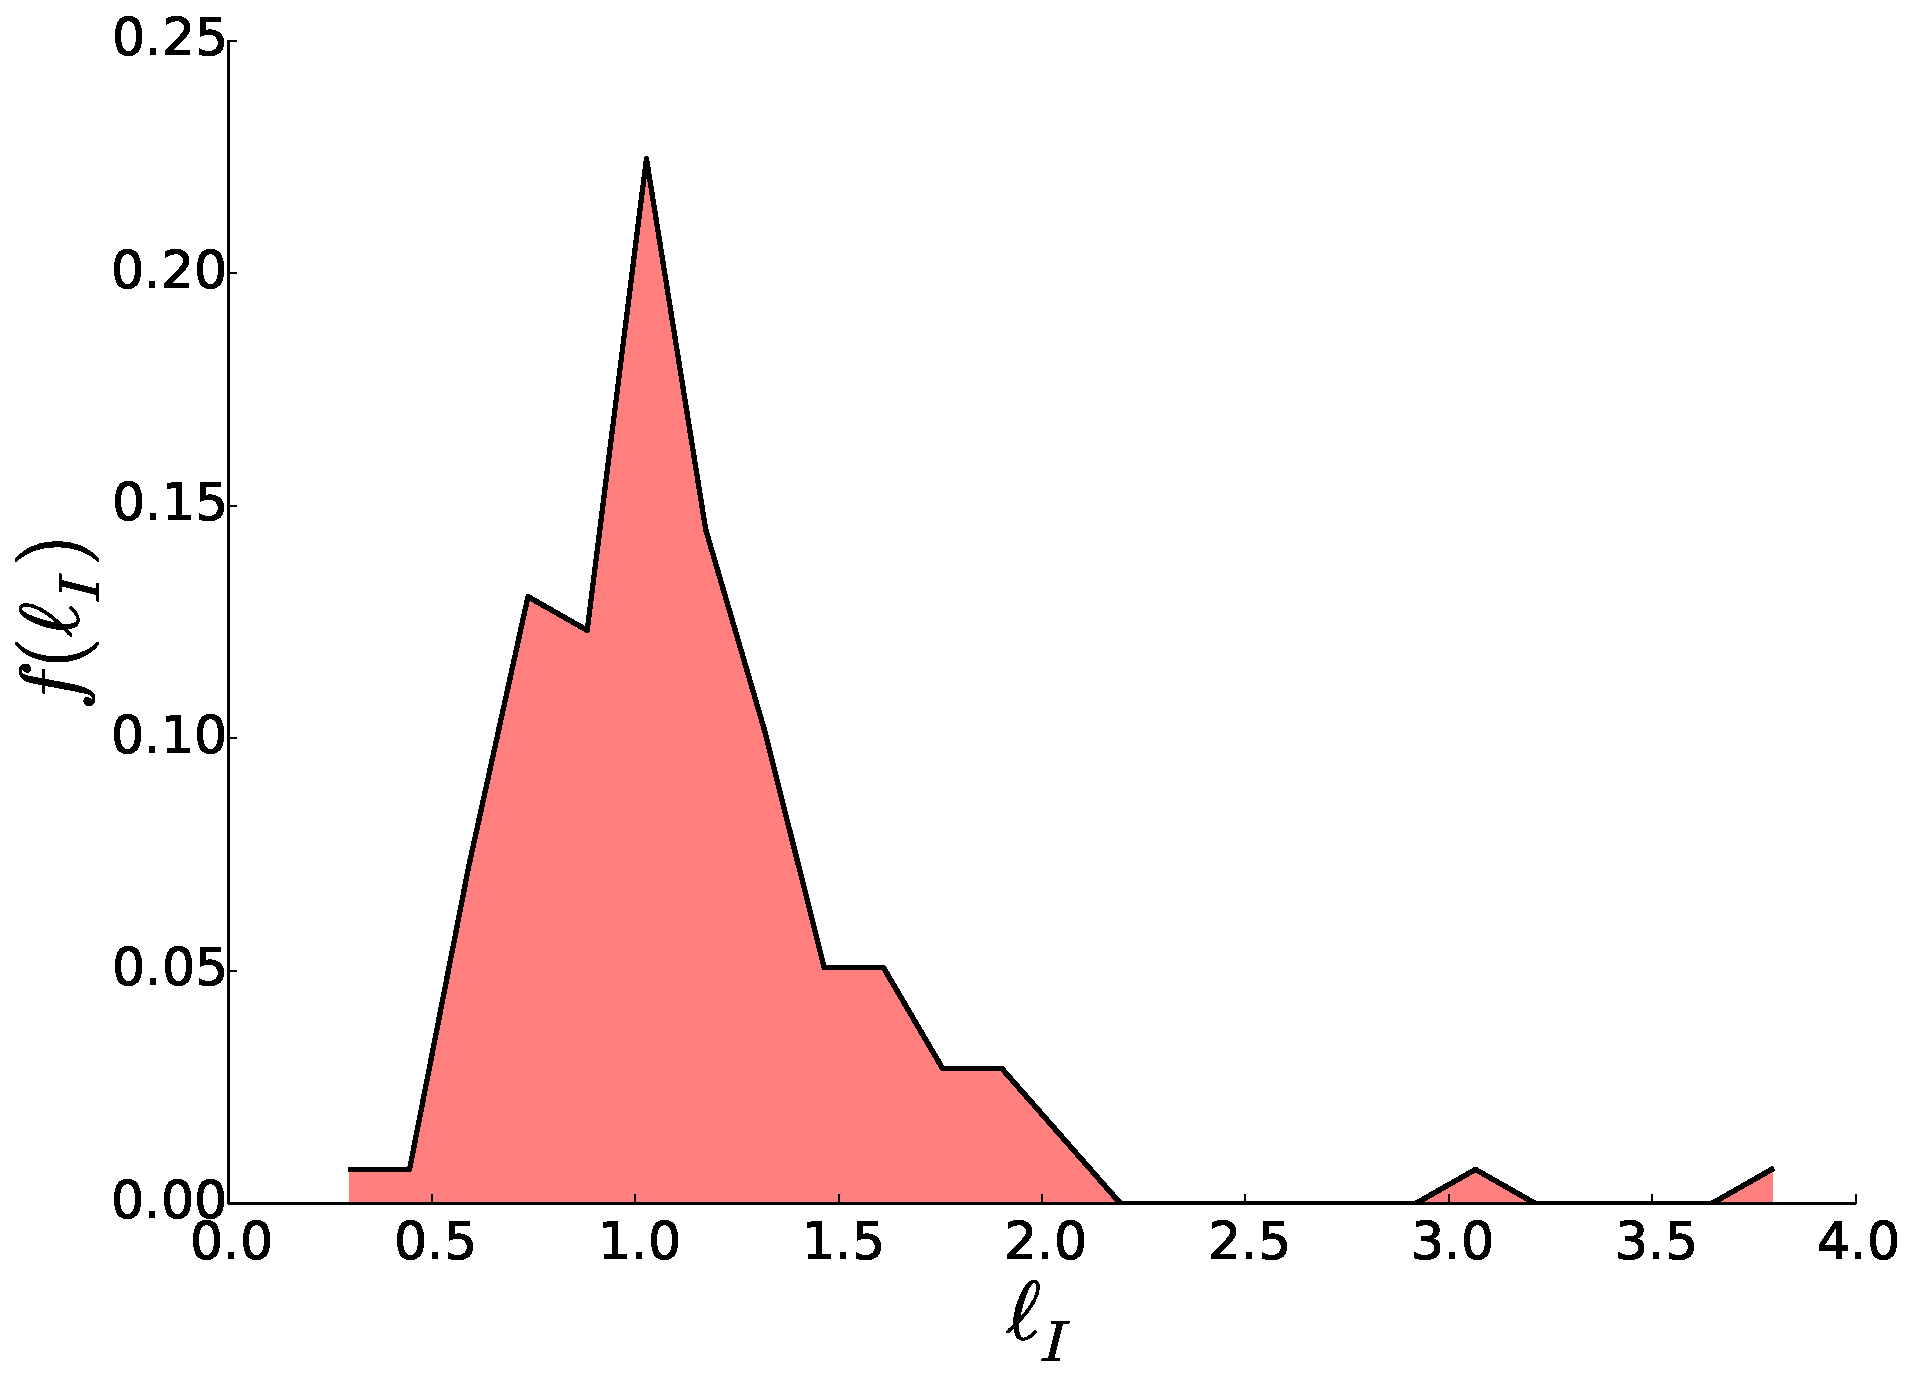
\includegraphics[width=0.49\textwidth]{gfx/chapter-networks/metro_hist_ell_1.pdf}
    \caption{{\bf (Subway) Relation between the length and the number of stations} (Left) Length of $138$ subway networks in the world as a function of the number of stations. A linear fit gives $L \sim 1.13\,N_S\,(R^2=0.93)$ (Right) Empirical distribution of the inter-station length. The average interstation distance is found to be $\overline{\ell_1} \approx 1.2\, \text{km}$ and the relative standard deviation is approximately $440\,\text{m}$ \label{fig:metro_length_stations}}
\end{figure}

As a result of the previous argument, we can express $\ell_1$ in terms of the systems characteristics. Indeed, the total ridership now reads

\begin{equation}
    R \sim \overline{\xi}\pi\rho\frac{L^2}{N_s}
    \label{eq:ridership-other}
\end{equation}

If we assume to be in the steady-state $Z_{sub} \approx 0$, using the results from Eqs.~(\ref{eq:cost-benefit},\ref{eq:ridership-other}), we find that the total length of the network and the number of stations are linked at first order in $\epsilon_s/\epsilon_L$ by

\begin{equation}
    L \sim \left( \frac{4 \epsilon_L}{\pi\,\xi\,f\,\rho} + \frac{\epsilon_s}{\epsilon_L}\right) N_s
    \label{eq:length-stations}
\end{equation}

and that the interstation distance reads

\begin{equation}
    \ell_1 = \frac{4 \epsilon_L}{\pi\,\xi\,f\,\rho} + \frac{\epsilon_s}{\epsilon_L}
\end{equation}

This relation implies that the interstation distance increases with an increased
station maintenance cost, and decreases with increased line maintenance costs,
density and fare. We thus see that the adjustment of $\ell_1$ to match $2\,d_0$
can be made through the fare price (or subsidies by the local authorities or
national government). At this point, it would be interesting to get reliable
data about the maintenance costs and fare for subway systems in order to pursue
in this direction and test the accuracy of this prediction.\\

So far, we have a relation between the total length and the number of stations,
but we need another equation in order to compute their value. Intuitively, it is
clear that the number of stations --- or equivalently the total length --- of a
subway system is an increasing function of the wealth of the city. We assume a
simple, linear relation of the form

\begin{equation}
    N_s = \beta \frac{G}{\epsilon_s}
\end{equation}

where $G$ is the city's Gross Metropolitan Product, and $\beta$ the fraction of
the city's wealth invested in public transportation. On
Fig.~\ref{fig:metro_stations_gdp} (left) we plot the number of stations of
different metro systems around the world as a function of the Gross Metropolitan
Product of the city. A linear fit agrees relatively well with the data
($R^2=0.73$, dashed line), and gives $\frac{\epsilon_s}{\beta} \approx
10^{10}\,\text{dollars/station}$. However, the dispersion around the linear
average behaviour is important: more specific data is needed in order to
investigate whether differences in the construction costs and investments (or
the age of the system) can, alone, explain the dispersion.

\begin{figure}
\centering
    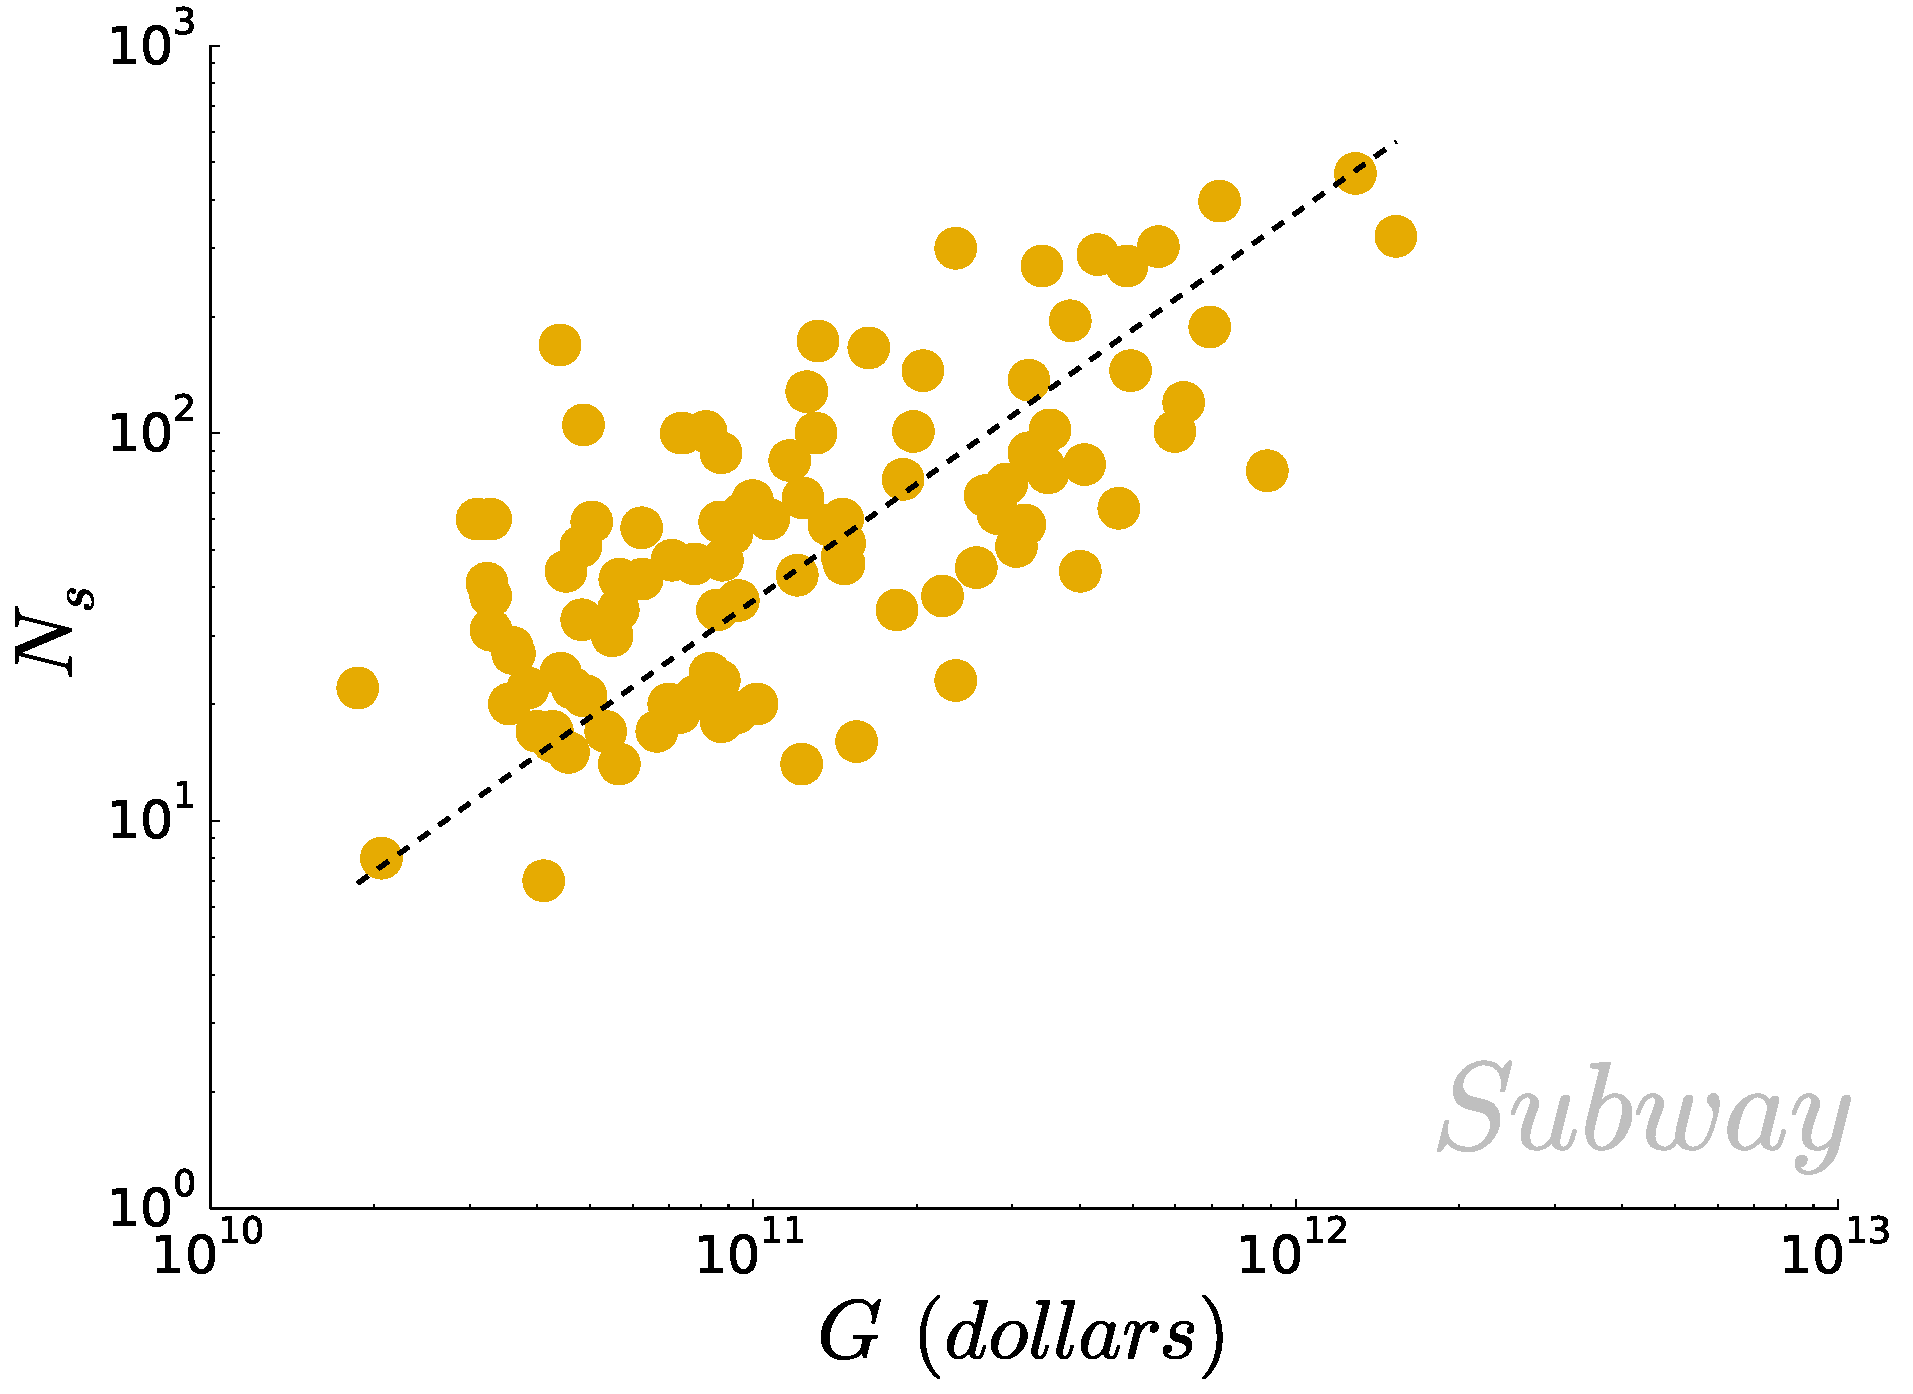
\includegraphics[width=0.49\textwidth]{gfx/chapter-networks/metro_stations_gdp.pdf}
    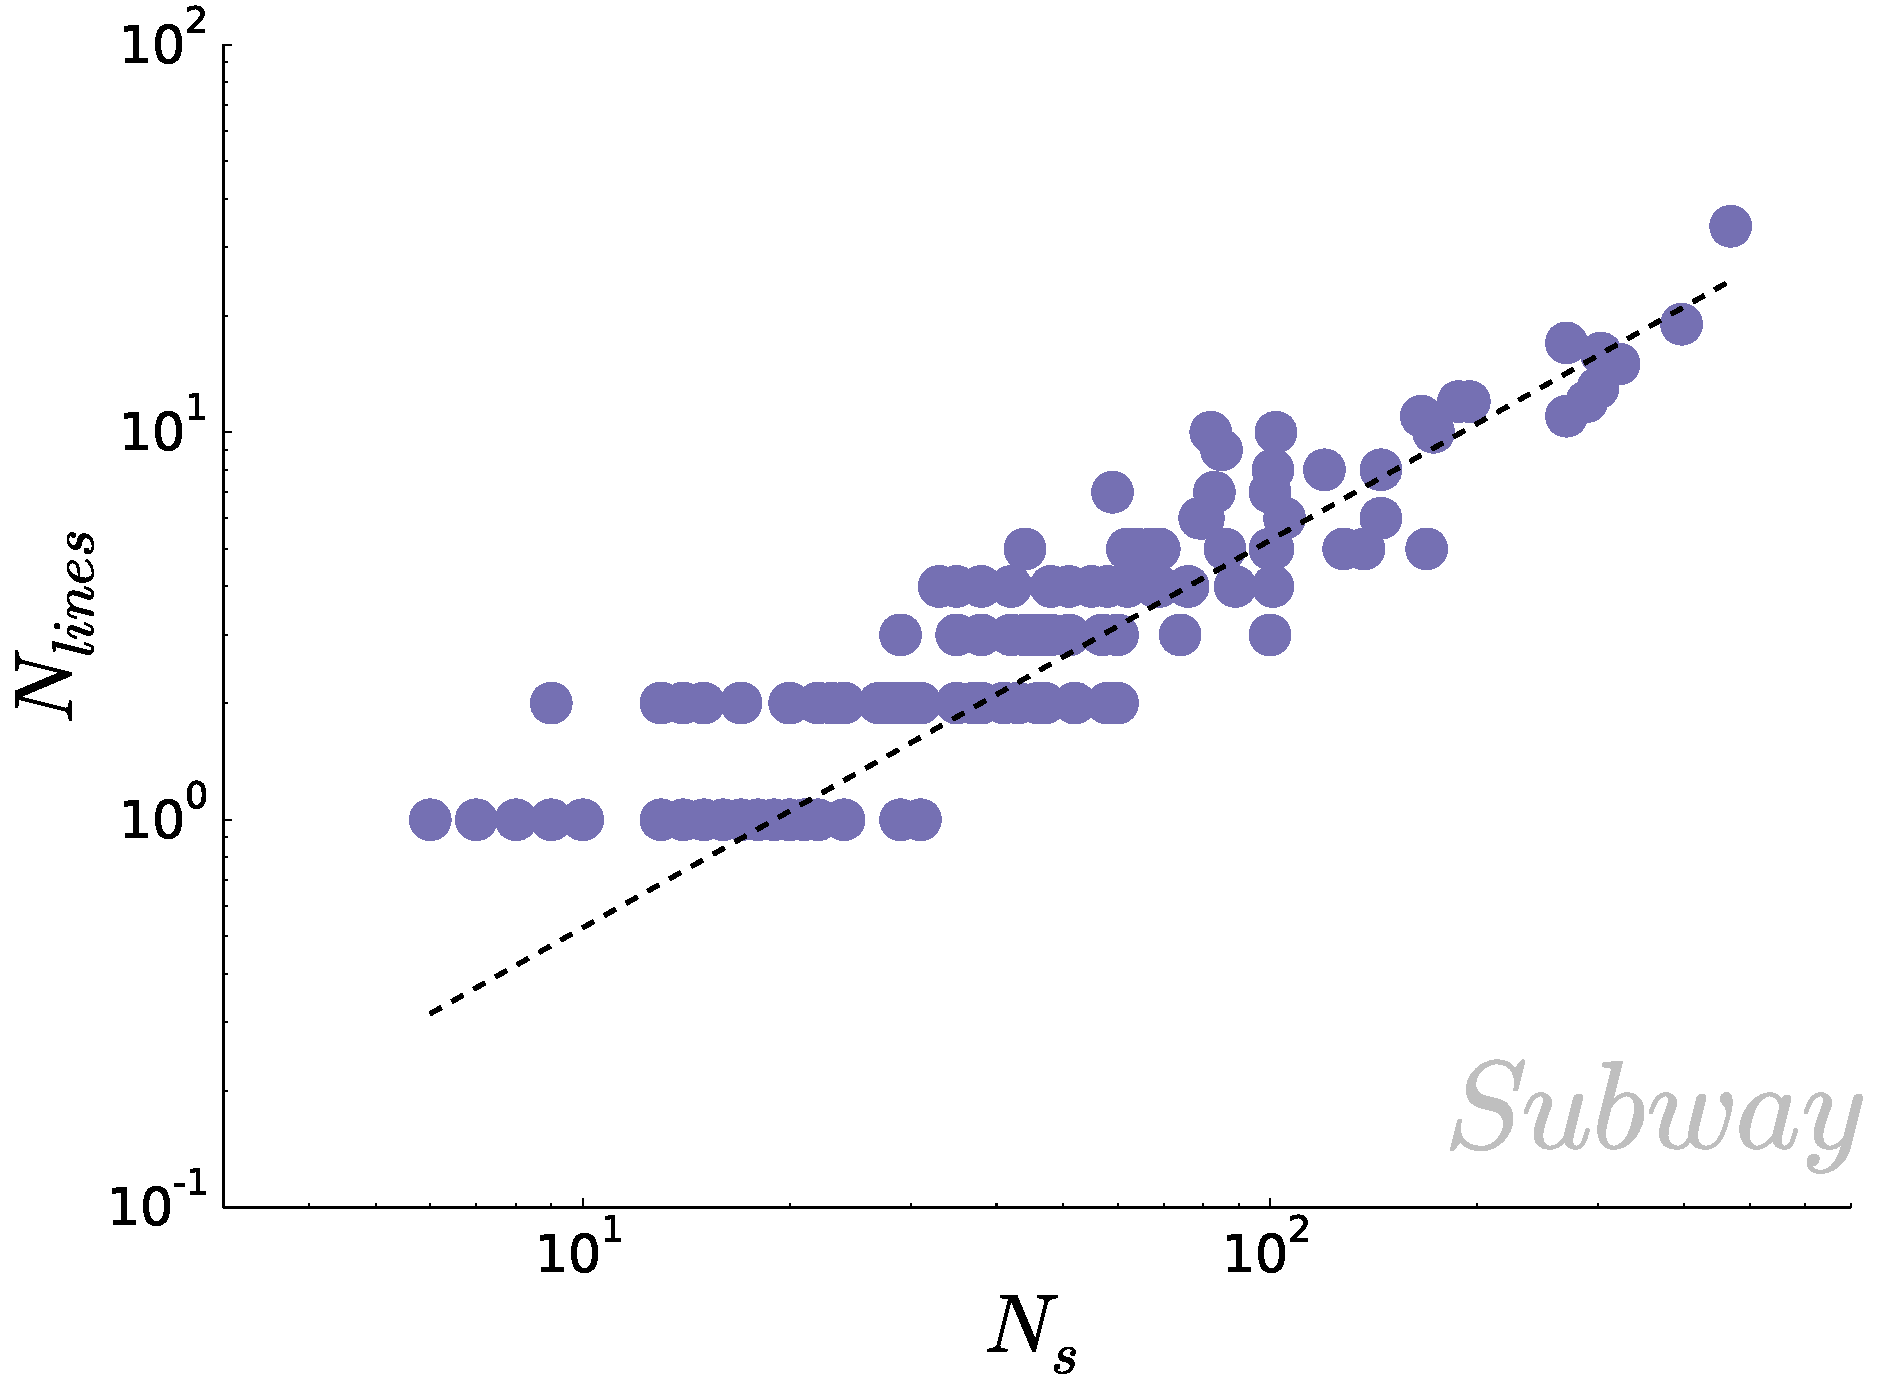
\includegraphics[width=0.49\textwidth]{gfx/chapter-networks/metro_lines_stations.pdf}
    \caption{{\bf (Subway) Size of the subway system and city's wealth} We plot the number of stations for the different subway systems in the dataset as a function of the Gross Metropolitan Product of the corresponding cities (obtained for $106$ subway systems). A linear fit (dashed line) gives $N_s = 2.51\, 10^{-10}\,G$ ($R^2=0.73$). {\bf (Subway) Number of lines and number of stations} We plot the number of metro lines $N_{lines}$ as a function of the number of stations $N_s$. A linear fit on the $138$ data points gives $N_{lines} \approx 0.053\,N_s\,(R^2=0.94)$, or, in other words, metro lines contain on average $19$ stations.}
    \label{fig:metro_stations_gdp}
\end{figure}

Finally, we now consider the number of different lines with distinct tracks. A
natural question is how the number of lines $N_{lines}$ scales with the number
stations $N_s$, that is to say whether lines get propotionally smaller, larger
or the same with the size of the whole system. We plot the number of lines as a
number of stations on Fig.~\ref{fig:metro_stations_gdp} and find that the data
agree with a linear relationship between both quantities ($R^2=0.93$, see the
dashed black line). In other words, the number of stations per line is
distributed around a typical value of $19$, whatever the size of the system.


\subsection*{Railway networks}

We start by discussing an important difference between railway and subway
networks. In the subway case, the interstation distance is such that it matches
human constraints: $\ell_1\sim 2\,d_0$ where $d_0$ is the typical distance that
one would walk to reach a subway station. For the railway network, the logic is
however different: while subways are built to allow people to move within a
dense urban environment, the purpose of building a railway is to connect
different cities in a country. In addition, due to the long distance and hence
high costs, it seems reasonable to assume that each station is connected to its
closest neighbour. In this respect, the railway network appears as a planar
graph connecting randomly distributed nodes in the plane in an economical way.
If we assume that a country has an area $A$ and $N_s$ train stations, the
typical distance between nearest stations will be

\begin{equation} 
    \ell_N = \sqrt{\frac{A}{N_s}} 
\end{equation}

The total length $L \sim N_s\,\ell_N$ is then given by

\begin{equation} 
    L \sim \sqrt{A\, N_s} 
\end{equation} 

In order to test this relation for different countries, we plot the adimensional
quantity $\frac{L}{\sqrt{A}}$ as a function of the number of stations $N_s$ on
Fig.~\ref{fig:length-stations}. A power law fit gives an exponent $0.50 \pm
0.08\,(R^2 = 0.87)$, which is consistent with the previous argument.

\begin{figure}
    \centering
    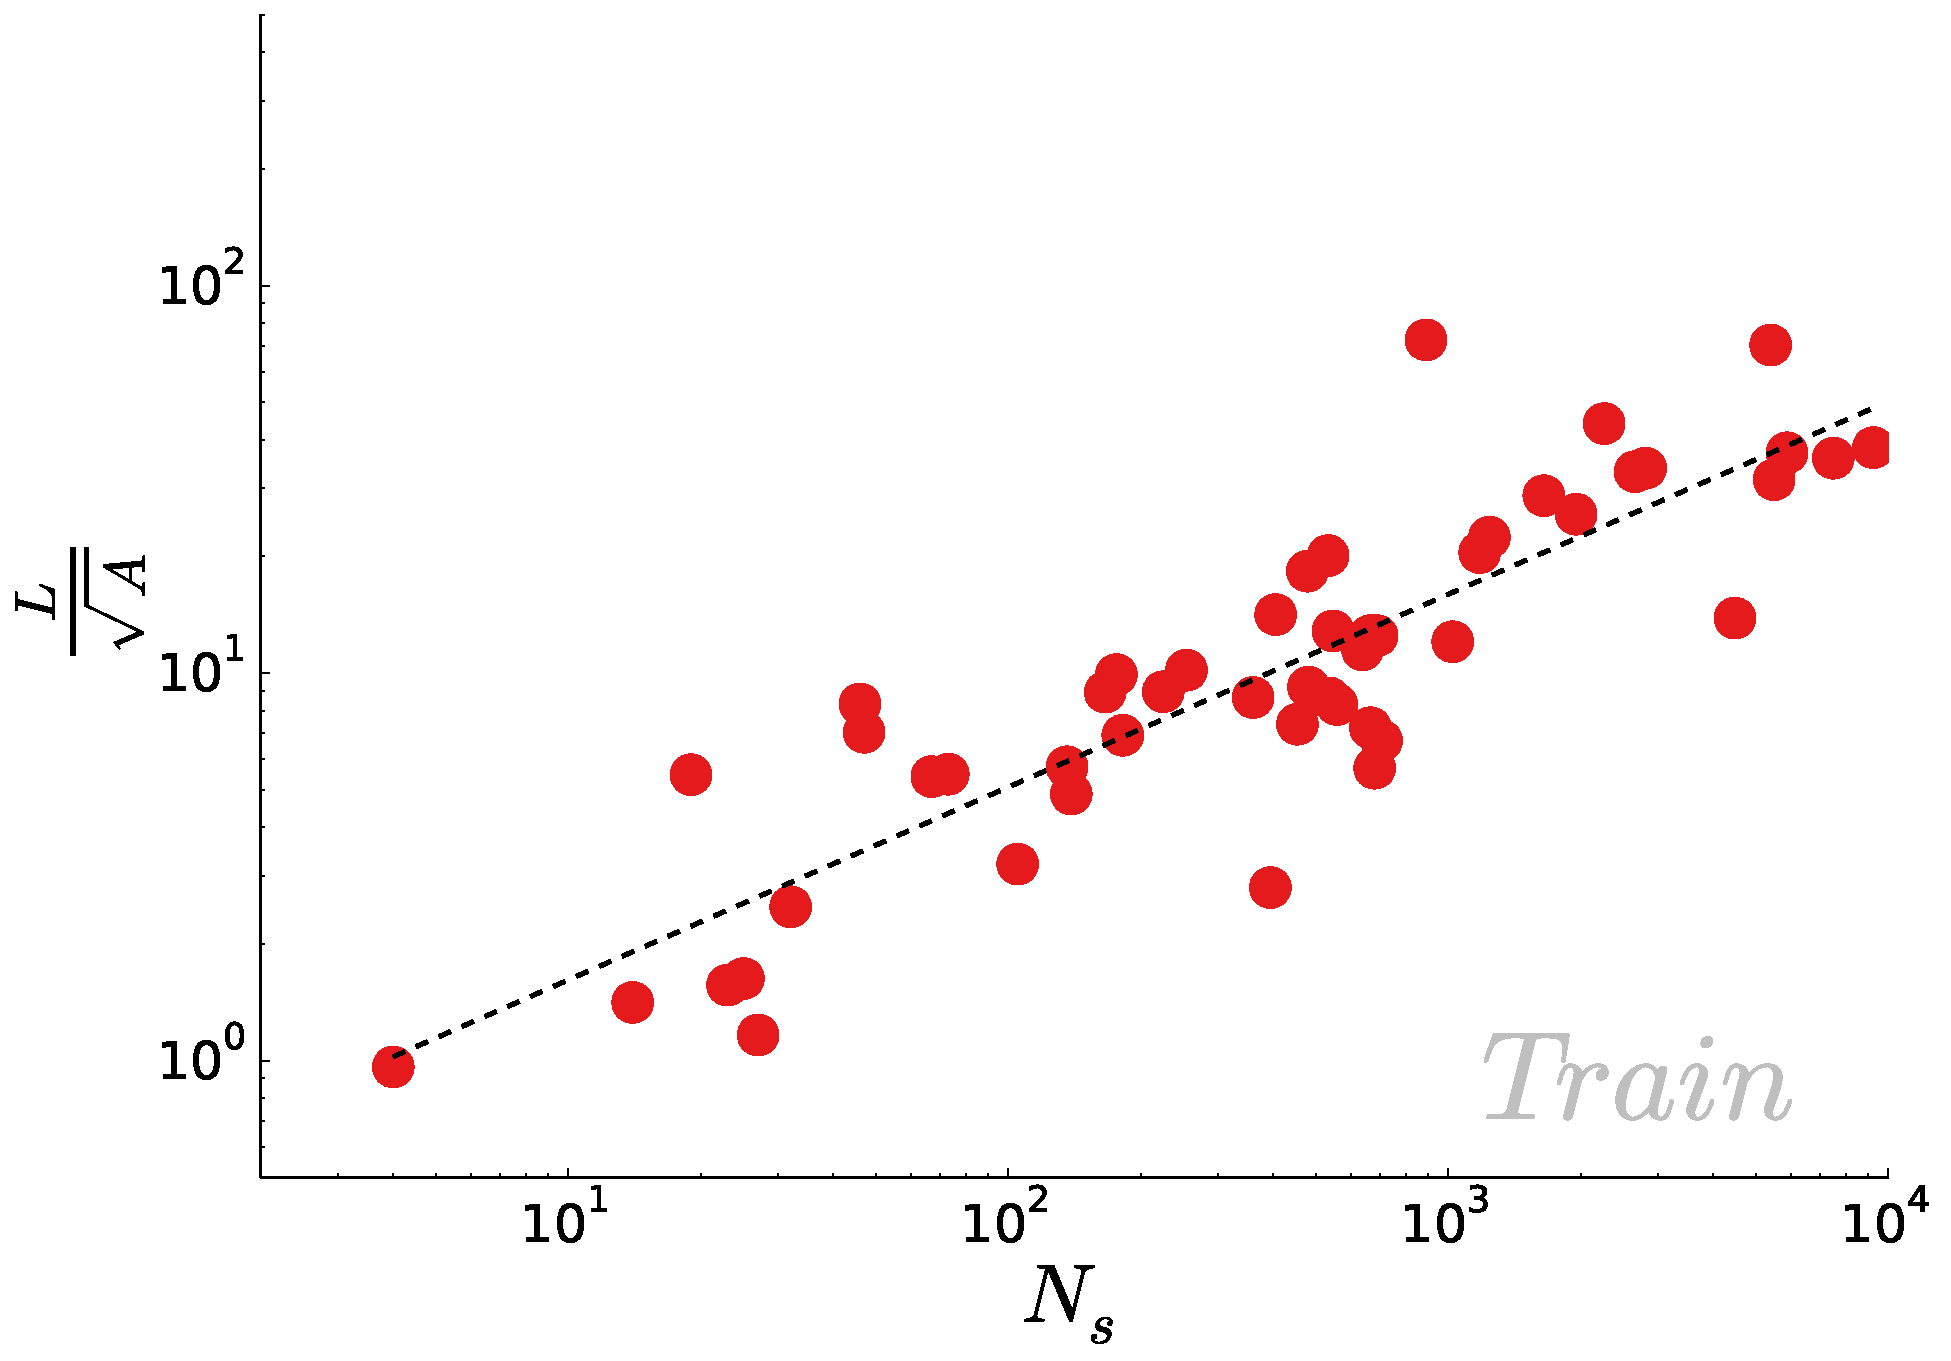
\includegraphics[width=0.5\textwidth]{gfx/chapter-networks/rail_length_stations.pdf}
    \caption{{\bf (Train) Total length and number of stations} Total length of the railway network $L$ rescaled by the typical size of the country $\sqrt{A}$ as a function of the number of stations $N_s$. The dashed line shows the best power-law fit on the $50$ data points with an exponent $0.50 \pm 0.08\,(R^2 = 0.87)$.\label{fig:length-stations}}
\end{figure}

At this point, we have a relation between $L$ and $N_s$, but we need to find the
expressions for the other quantities. There are other differences with the
subway system. First, due to the distances involved, the ticket price usually
depends on the distance travelled and we will denote by $f_L$ the ticket price
per unit distance. The relevant quantity for benefits is therefore not the raw
number of passengers--as in subways--, but rather the total distance travelled
on the network $T$. Also, again due to the long distances spanned by the
network, the costs of stations can be neglected as a first approximation, and we
get for the budget the following expression

\begin{equation}
    Z_{train} \simeq T\, f_L - \epsilon_L\, L
\end{equation}

In the steady-state regime $Z_{train}\approx 0$ --- or in other words, the
revenue generated by the network use must be of the order of the total
maintenance costs~\cite{Louf:2013} --- we find that

\begin{equation}
    T \sim \frac{\epsilon_L}{f_L} L
\end{equation}

In addition, if we assume that the order of magnitude of a trip is given by
$\ell_N$, the total travelled length is simply proportional to the ridership
$T\sim \ell_N R$ leading to 

\begin{equation}
    R \sim \frac{\epsilon_LN_s}{f_L}
\end{equation}

We thus plot the total daily ridership $R$ as a function of the total number of
stations $N_s$ (figure \ref{fig:train_rider}), and despite the small number of
available data points, a linear relationship between these both quantities seems
to agree with empirical data on average ($R^2 = 0.86$). This result should be
taken with caution, however, due to the important dispersion that is observed
around the average behaviour, and the small number of observations.

\begin{figure}
    \centering
    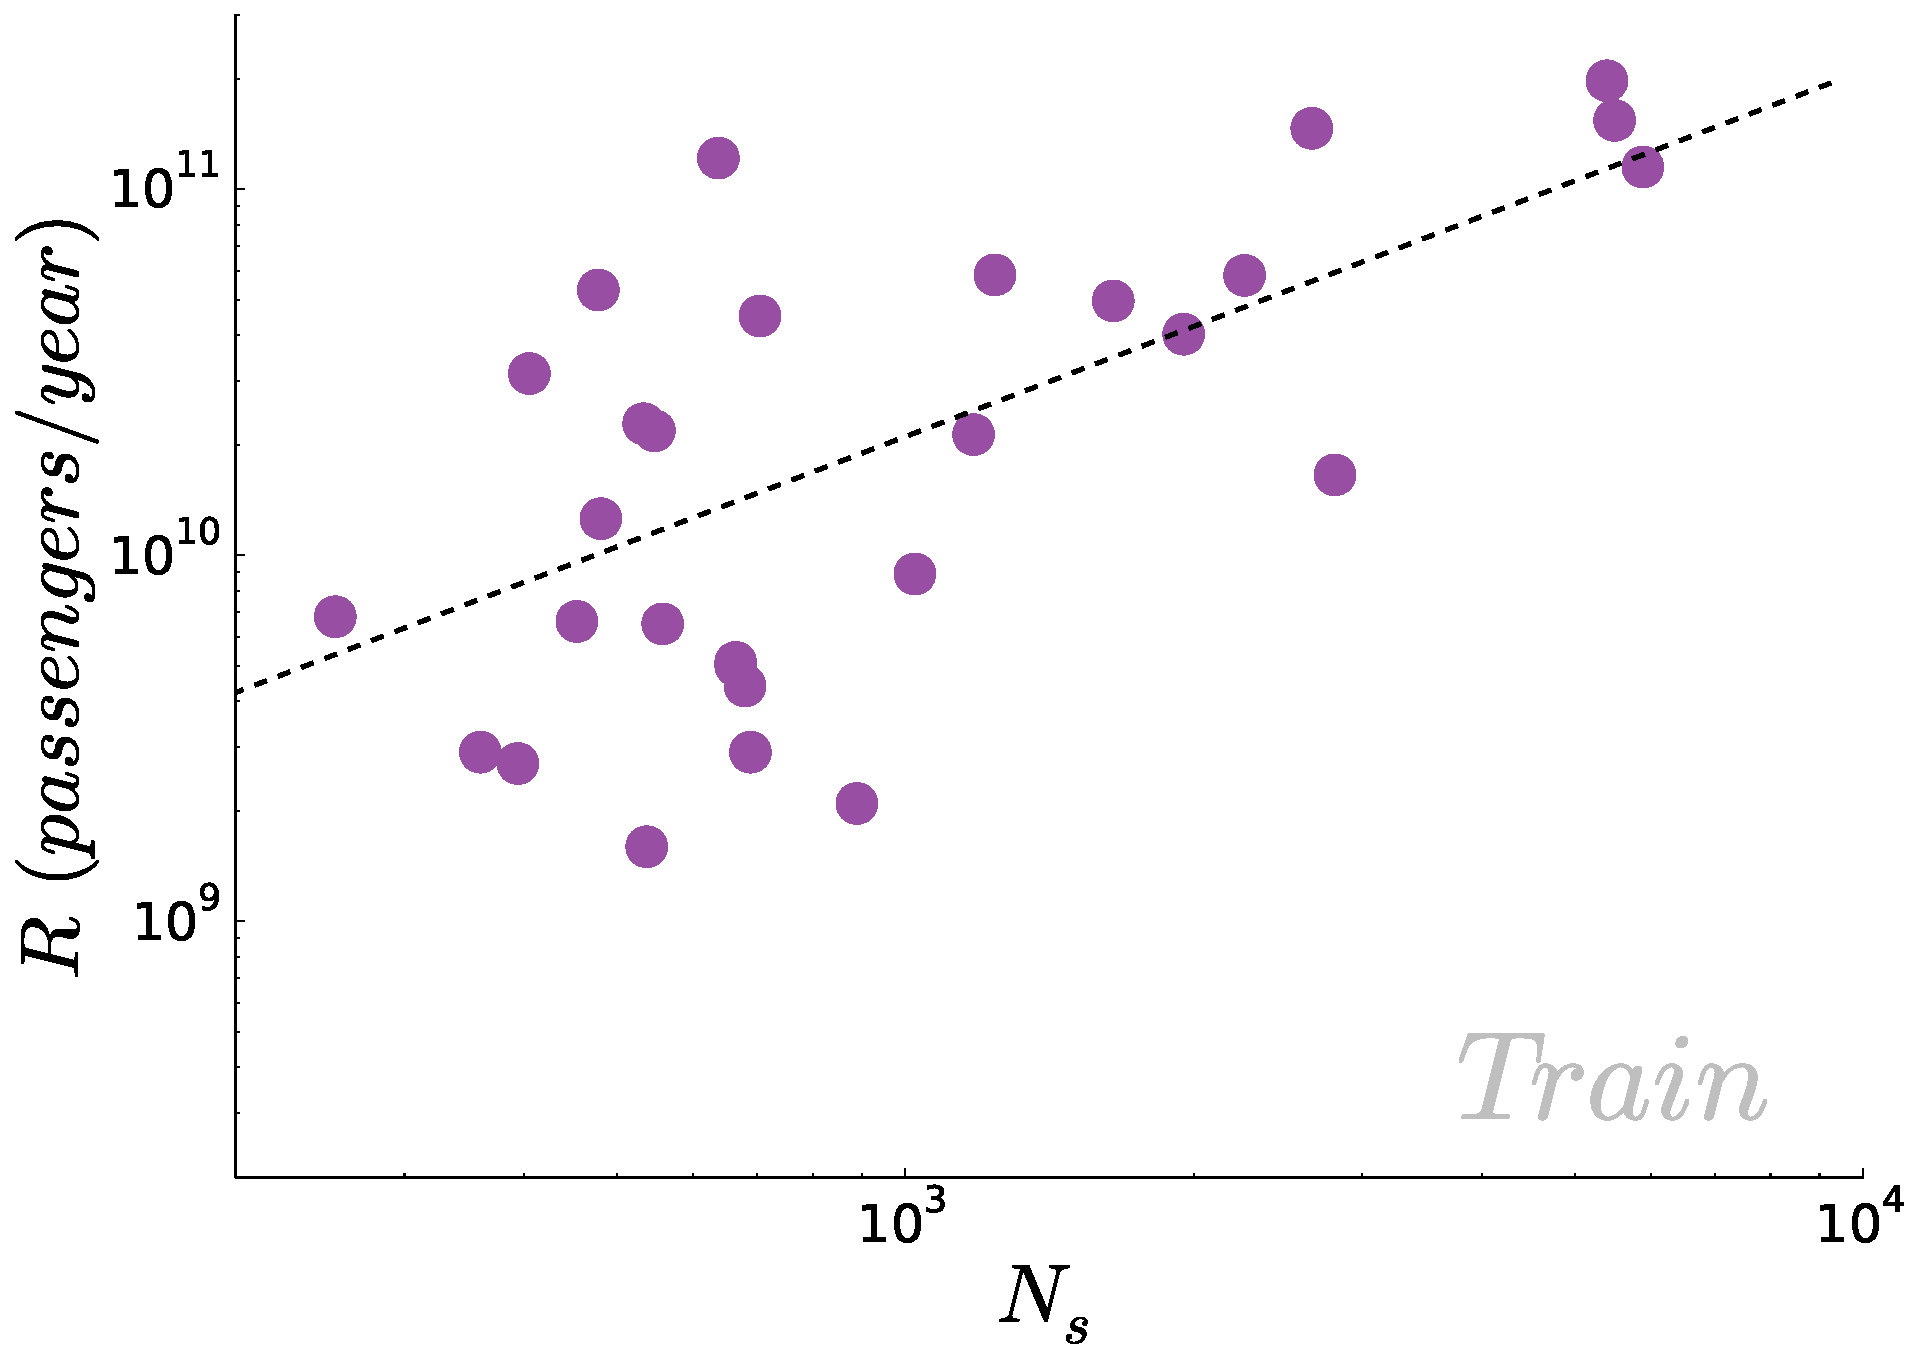
\includegraphics[width=0.5\textwidth]{gfx/chapter-networks/rail_ridership_stations.pdf}
    \caption{{\bf(Train) Ridership and number of stations} The total yearly ridership $R$ of the railway networks as a function of the number of stations. A linear fit on the $47$ data points gives $R \sim 7.0\,10^8\:N_s$ ($R^2 = 0.86$)}
\label{fig:train_rider}
\end{figure}

According to the previous result, the total length and the number of stations
are related to each other. We now would like to understand what property of the
underlying country determines the total length of the network. That is to say,
why networks are longer in some countries than in others. As in subway systems,
economical reasons seem appealing. Indeed, the railway networks of some large
african countries such as Nigeria are way smaller than that of countries such as
France or the UK of similar surface areas. A priori, when estimating the cost of
a railway network, one should take into account both the costs of building lines
and the stations. However, as stated above, considering the distances involved,
the cost of building a station is negligible compared to that of building the
actual lines. We thus can reasonably expect to have

\begin{equation} L \sim \frac{\alpha\,G}{\epsilon_L} \end{equation}

where $G$ is here the country's Gross Domestic Product (GDP) used as an
indicator of the country's wealth, and $\alpha < 1$ the ratio of the GDP
invested in railway transportation. We plot $L$ as a function of $G$ on
Fig.~\ref{fig:length-gdp} and the data agree well ($R^2 = 0.91$) with a linear
dependence between $L$ and $G$. Again, the dispersion indicates that the linear
trend should only be understood as an average behaviour and that local
particularities can have a strong impact on the important deviations observed.
For instance, the United Arab Emirates are far from the average behaviour, with
a $52\,\text{km}$ network and a GDP of roughly $3\,10^5$ million dollars. Yet,
the construction of a $1,200\,\text{km}$ railway network has been decided in
2010, which would bring the country closer to the average behaviour. 

\begin{figure}
    \centering
    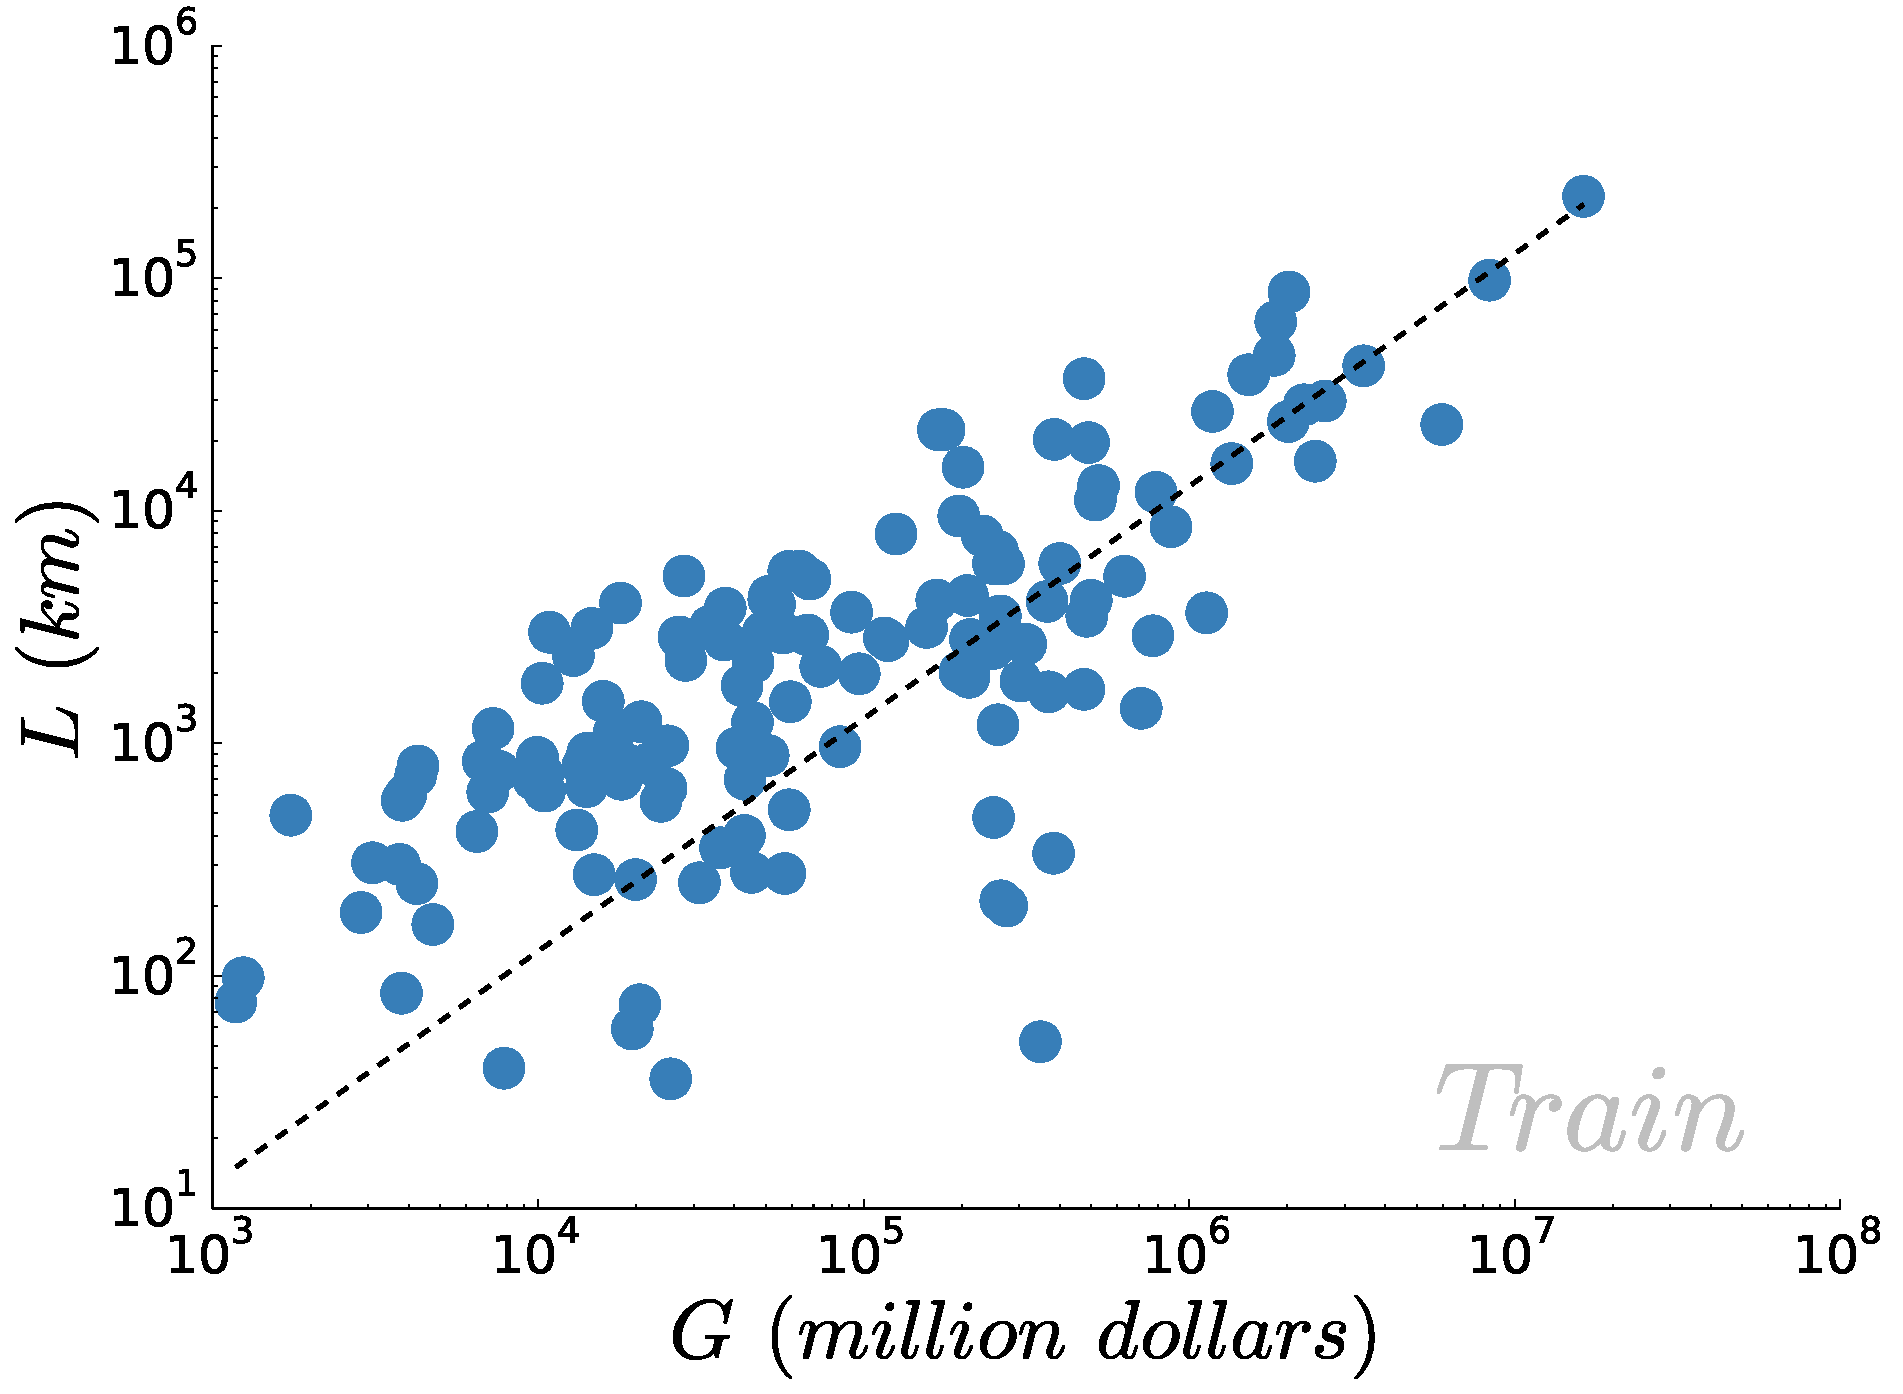
\includegraphics[width=0.5\textwidth]{gfx/chapter-networks/rail_length_gdp.pdf}
    \caption{{\bf(Train) Total length of the network and wealth} Total length of the railway network $L$ as a function of the country GDP $G$. The dashed line shows the best linear fit on the $138$ data points which gives $\epsilon_L / \alpha \approx 10^4\, \text{dollars.km}^{-1}\,(R^2 = 0.91)$.\label{fig:length-gdp}}
\end{figure}

\section*{Discussion}

We have proposed a general framework to connect the properties of railway and
subway systems (ridership, total length and number of stations) to the
socio-economic and spatial characteristics of the country or city they are built
in (population, area, GDP). Despite their simplicity, our arguments agree
satisfactorily with the data we gathered for more than $100$ subway systems and
$50$ railway networks accross the world. It should be noted that the noise
associated with these data (and sometimes their definition, see Material and
Methods) makes it difficult to infer behaviours from the empirical analysis
alone. Therefore, the most appropriate way to proceed, we believe, is to make
assumptions about the systems and build a model whose predictions can then be
tested against data.

This study suggests that the fundamental difference between railways and subways
comes from the determination of the interstation distance. While it is imposed
by human constraints in the subway case, the railway network has to adapt to the
spatial distribution of cities in a country. This remark is at the heart of the
different behaviors observed for railways and subways (see
Table~\ref{table:summary} for a summary of these differences). 

The previous arguments are able to explain the average behaviour of various
quantities. Nevertheless, it would be interesting to identify deviations from
these behaviours, and see whether they correlate --for instance-- with
topological properties of the system, as suggested in~\cite{Derrible:2009} or
other properties of the network and the region. We think that the relations
presented here provide  nevertheless a simple framework within which local
particularities can be discussed and understood. We also think that this
framework could be used as a useful null-model to quantify the efficiency of
individual transportation networks, and compare them to each other. This would
however require more specific data than those that were available to us. 

While we have focused on an average, static description of metro systems, we
believe that our study provides a better understanding of how these systems
interact with the region they serve. This new insight is a necessary step
towards a model for the growth of subway systems that takes the characteristics
of the city into account. Indeed, although models of network growth exist, the
length of networks and nodes at a given time is usually imposed exogeneously,
instead of being linked to the socio-economic properties of the substrate. This
study provides a simple approach to these complex problems and could help in
building more realistic models, with less exogeneous parameters.

It would be interesting to gather data about the exact structure of all the
studied network, so as to study whether there is a relationship between the
topology (degree distribution, detour index, etc.) of these networks and
properties of the substrate, as was done for the road network
in~\cite{Levinson:2012}.

Finally, gathering historical data should allow to address the problem of the
conditions for the appearance of a subway in a city. In particular, we observe
empirically that the GDP of the cities that have a subway system is always
larger than about $10^{10}$ dollars, a fact that calls for a theoretical
explanation. 


% You may title this section "Methods" or "Models". 
% "Models" is not a valid title for PLoS ONE authors. However, PLoS ONE
% authors may use "Analysis" 

\section*{Materials and Methods}

Data for $138$ subways accross the world were mainly collected on Wikipedia~\cite{Wiki}, and cross-referenced with the operators' data when possible. The cities' GDP per capita was retrieved for $114$ cities from Brooking's Global MetroMonitor~\cite{Brookings}. The choice of population and city area was more subtle. Indeed, most subway systems span an area greater than the city core, and the relevant area therefore lies somewhere between the city core's area and the total urbanized area. We chose to use the population and surface area data for urbanized areas provided by Demographia~\cite{Demographia}.

While data about ridership, network length were easily retrievable for more than $100$ countries from the UIC Railisa 2011 database~\cite{railisa}, data about the number of stations were more difficult to find. We had to use various data sources, mainly scrapping the operators' ticket booking websites. Data about the GDP, population and surface areas of different countries were obtained from the World Bank~\cite{WorldBank}, and the United Nations Statistics Division~\cite{UnitedNations}.\\

All the data used for this study are publicly available in tsv format at~\cite{data_repo}.


\section*{Tables}
\begin{table}[!ht]
\centering
\begin{tabular}{|c|c|c|}
\hline
 & {\bf Subway} & {\bf Train} \\
 \hline
$L / N_s$ & cste. & $\sqrt{\frac{A}{N_s}}$\\
$R$ & $\frac{P}{A}\,N_s$ & $N_s$ \\
$G$ & $N_s$ & $L$ \\
\hline
\end{tabular}
\caption{{\bf Summary of the differences between subways and railways}
We summarize the difference of behaviour between subways and railways. The
scaling of the length $L$ of the network with the number of stations $N_s$
reveals the different logics behind the growth of these systems. Another
difference lies in the total ridership $R$: while it depends on the population
density $P/A$ for subways, it only depends on the number of stations $N_s$ for
train networks. Finally, the size of both types of network can be expressed as a
function of the wealth of the region, represented here by the GDP $G$. However,
because the interstation length is constant for subways, the size is better
expressed in terms of the number of stations $N_s$; in the case of railway
networks, the cost of stations are negligible compared to the building cost of
lines, and the size is better expressed in terms of the total length $L$.
\label{table:summary}} 
\label{tab:label} 
\end{table}
